\chapter{Monad Transformers}
\section{Overview}

As we already have monad designed to model side-effect with restricted type,it would not be too much problem to perform an action using monad in Haskell.New monad might be needed form operation that are able to perform state manipulation as well as IO action.\\

Monad transformers offer an additional benefit to monadic programming: by providing a
library of different monads and types and functions for combining these monads, it is possible
to create custom monads simply by composing the necessary monad transformers. \cite{step} \\

In real world application, it is often the case that a combination different type of action is required to put into one function.Monad transformer provide a new way to glue them together.

\section{State Transformer}
A value of type \textbf{(ST a s)} is a computation which transforms a state index by type s ,and delivers a value of type a ,You can think of it as a box ,like this 
\begin{figure}[H]
  \centering
	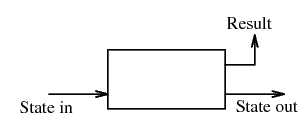
\includegraphics[width=0.60\textwidth]{pic/c3/state.png}
	\caption{Diagram illustrating a state monad}
\end{figure}\cite{lazy1}
\\

First , a state transformer is a monad, other than encapsulating a data behind signature , it encapsulated a computation,the \textbf{runState} function provide by the state monad is an escape function that allow us to extract is state logic from the computation,by feeding the state computation function with an initial state,we are able to get the final state.Other type of escape function is provided to extract computation as well.

Second,a state transformer can accept other monads to combine the computation which state as well as other logic says the IO logic.


\section{Error Transformer}
ErrorT monad transformer can be used to add error handling to another monad.
The ErrorT monad type constructor is ,
\begin{hcode}
newtype ErrorT e m a
\end{hcode}
The first parameter e is the error type like the Either Monad constructor ,m is the inner monad,a is the type of the computation.

\begin{hcode}
instance (Monad m, Error e) => Monad (ErrorT e m) where
    return a = ErrorT $ return (Right a)
    m >>= k  = ErrorT $ do
        a <- runErrorT m
        case a of
            Left  l -> return (Left l)
            Right r -> runErrorT (k r)
\end{hcode}

From the definition above , we can derive its bind strategy which is the most important thing for us to understand a monad.For two computation \textbf{m} and {k},the bind strategy is  that it will try to extract the result from the first computation which might return a error message ,the whole computation will fail on the first computation which will attempt on the succeed of the first.computation.

The escape function \textbf{runErrorT} can help us to extract the inner level monad which is a computation with some kinds of monad logic and execute it.


\begin{hcode}
getValidPassword :: ErrorT String IO String
getValidPassword = do s <- lift getLine
                      guard (isValid s)
                      return s
                      	where isValid = (>5).length
 
askPassword :: ErrorT String IO ()
askPassword = do lift $ putStrLn "Insert your new password:"
                 value <- getValidPassword
                 lift $ putStrLn "your password is valid"
                              
runProgram = runErrorT askpassword                
\end{hcode}

The code above shows how a problem written by Error transformer \textbf{ErrorT} combines error handling as well as IO action.The runErrorT will extract the message which is either left value of right value.By combining\\ \textbf{getValidPassword} together with lifted IO action,the logic that the string "your password is valid" will not return if user's input string is shorter than 5 has been implemented easily an elegantly because the bind operating itself implies failure values bypass the follow computation.

\section{Combining Monads}
Monad transformers create a new monad by extending an existing monad with additional operations, thereby allowing new programming language features to be de defined while preserving any language definition given for the original monad.\cite{modular} \\ 

As monad guarantees the correctness of the computation with the type restriction,namely we can not combine two computations one with "stateful" while other with IO logic into one building block,we might need addition functions like lift and liftIO together with monad transformer to fix the type problem .\\


As we can imagine that, if could combine every monad for most of monad if offer a monad transformer form.In this way,the action combine inside to notation would probably be no different from a real imperative language.When we combine all monads, the type restricted become slacked accepting a type of computation with side effect which is no difference from a real imperative language.\\

The only difference might be the sequence we encapsulate monad and monad transformers,that is we can only warp IO inside other monad transformers.
